\documentclass{standalone}

\usepackage{tikz}
\usetikzlibrary{arrows}
\usetikzlibrary{decorations.pathmorphing,patterns}

\begin{document}
  

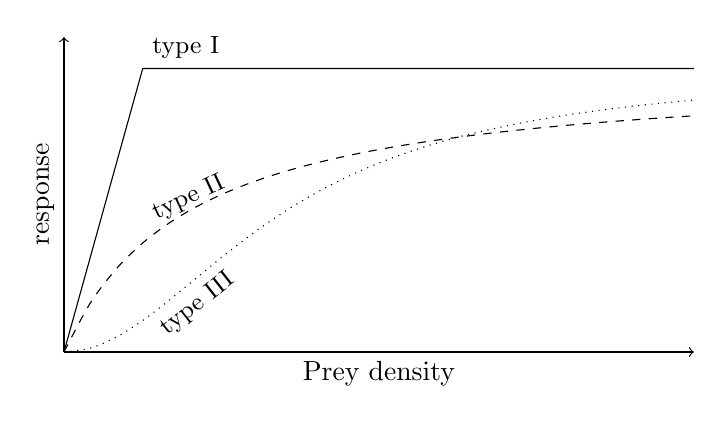
\begin{tikzpicture}[xscale=2,yscale=4]

  \draw[->] (0,0) -- (4,0);
  \draw (2,0)node[below]{Prey density};
  \draw[->] (0,0) -- node[pos=.5,rotate=90,above]{response}(0,1);
  \draw (0,.5) ;
  \draw (0,0) -- (.5,.9) -- node[pos=0,above right]{\small type I}(4,.9);
  \draw[smooth, domain=0:4,dashed] plot(\x,{.9*\x/(\x+.8)});
  \node[above right=4pt,rotate=25] at (.5,.33) {\small type II};
  \draw[smooth,domain=0:4,dotted] plot(\x,{.9*\x^2/(\x^2+2)});
  \node[below right,rotate=38] at (.5,.1) {\small type III};

\end{tikzpicture}

\end{document}
